%! program = pdflatex

\documentclass[11pt,a4paper]{article}
\usepackage{geometry} % see geometry.pdf on how to lay out the page. There's lots.
\geometry{a4paper} % or letter or a5paper or ... etc
% \geometry{landscape} % rotated page geometry
\usepackage{graphicx}
% See the ``Article customise'' template for come common customisations
\input{pic-common}

\title{Precision recall curves}
\author{Peter Corke}
\date{December 2016} % delete this line to display the current date

\newcommand{\TP}{\mbox{TP}}
\newcommand{\FP}{\mbox{FP}}
\newcommand{\TN}{\mbox{TN}}
\newcommand{\FN}{\mbox{FN}}
\newcommand{\TPR}{\mbox{TPR}}
\newcommand{\FPR}{\mbox{FPR}}
\newcommand{\TNR}{\mbox{TNR}}

\newcommand{\SPC}{\mbox{SPC}}

%%% BEGIN DOCUMENT
\begin{document}

\maketitle

\section{Binary classifiers}
Binary classifiers are widely used in fields as diverse as document retrieval and robot navigation.
We will first consider a familiar case of document retrieval using a tool like Google where we perform a search and expect to see only relevant documents.  The classifier, Google in this case, will:
\begin{itemize}
\item  return a relevant document  (true positive)
\item return an irrelevant document (false positive)
\item choose not to return a relevant document  (false negative)
\item chooses not to return an irrelevant document (true negative)
\end{itemize}
If we consider that the classification of the document is either positive (relevant) or negative (not relevant) then we can express these four outcomes
in  a $2 \times 2$ contingency table or confusion matrix as shown in Figure \ref{fig:confusion}.
We introduce the common shorthand notation TP, FP, FN and TN.
The two error situations FP and FN are often referred to as type I and type II errors respectively.  False positives or type I errors are also referred to as false alarms.
The number of relevant documents is $TP+FN$ and the number of irrelevant documents is $TN+FP$.

\begin{figure}
\centering
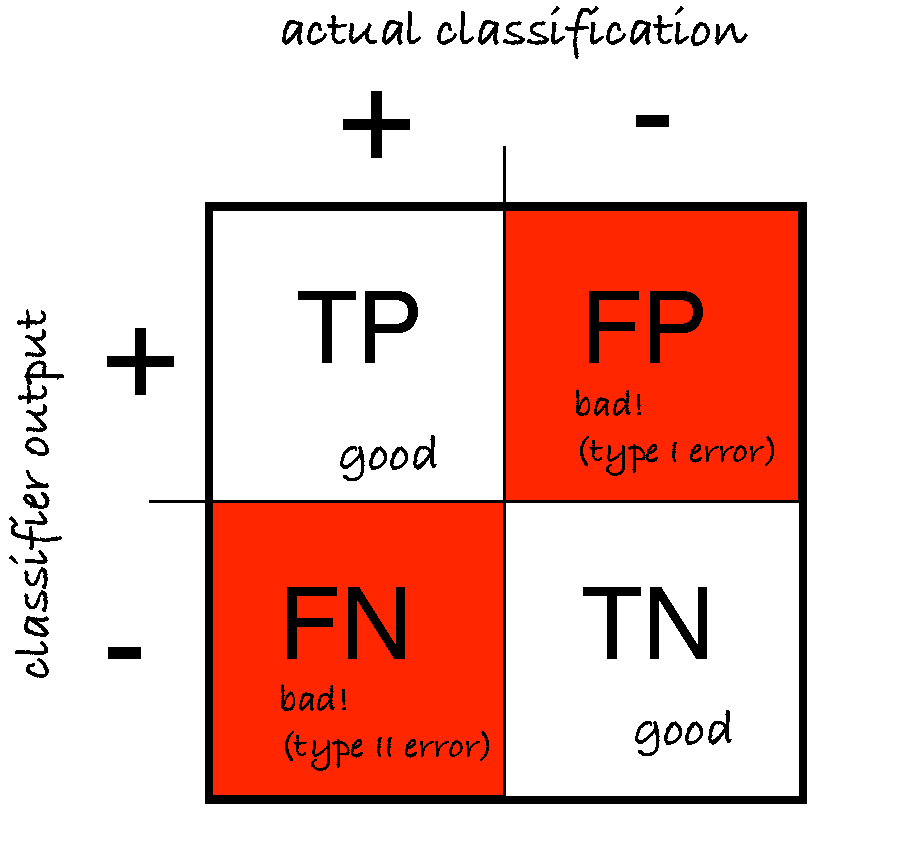
\includegraphics[width=0.6\textwidth]{confusion}
\caption{Confusion matrix for a binary classifier which maps the true classification against the output of the classifier.}
\label{fig:confusion}
\end{figure}

Consider now a robot localization problem.  The  robot is at a particular point X and its localizer can do one of four things:
\begin{itemize}
\item correctly report the robot is at  X (true positive)
\item incorrectly report the robot is at X  (false positive)
\item incorrectly report the robot is not at X (false negative)
\item correctly report the robot is not at X  (true negative)
\end{itemize}
For robot navigation we need to determine what it means to be ``at location X'' given the inevitable errors in sensor data that lead to uncertainty in location.  Typically there
is some threshold test that depends on the scale of the environment.  For FABMAP\cite{fabmap} and SeqSLAM\cite{seqslam} (and its derivatives) this is 40\unit{m}.

\subsection{Accuracy}
Accuracy is the number of correct classifications as a fraction of all classifications.
It is the sum of the diagonals of the confusion matrix divided by the total
 \[
\mbox{Acc} = \frac{\TP+\TN}{\TP+\FP+\TN+\FN}
 \]
 
 However for the case of imbalanced classes, that is, where one of the classes is very unlikely this measure can be very misleading.
Consider the case of classifying airline passengers as a terrorist (T) or not-a-terrorist (NaT) \cite{Koehrsen}.
For the period 2000--17 there were 800M passengers per year and only 19 confirmed terrorists.
A classifier that declared everybody as NaT would have 

\begin{table}[h]
\centering
\begin{tabular}{|l|l|l|} \hline
TP & T classified as T &  0 \\
TN & NaT classified as NaT & $18 \times 800\times 10^6$  \\
FP & NaT classified as T & 0 \\
FN & T classified as NaT &  19 \\  \hline
\end{tabular}
\end{table}

Accuracy in this case is 
\[
\frac{18 \times 800\times 10^6}{18 \times 800\times 10^6 + 19} \approx 99.9999999\%
\]
which is very good, but misses the point of being useful since it would not detect a single terrorist.


\section{Precision and recall}
For a particular experiment (over a number of documents or a number of points along the robot's path) where we know the true classification, we can compute the number of instances of 
each element in the table shown in Figure \ref{fig:confusion}.
From these four numbers we can compute a number of performance measures:
\begin{itemize}
\item Precision is the fraction of retrieved documents that are relevant, or the fraction of localizations that are correct
 \[
 P = \frac{\TP}{\TP+\FP}
 \]

\item Recall is the fraction of relevant documents that are retrieved, or the fraction of correct localizations that are given
 \[
 R = \frac{\TP}{\TP+\FN}
 \]
\end{itemize}

A classifier with high precision gives very few incorrect answers.  For information retrieval this means very few irrelevant documents are returned, while for localization this means very few incorrect locations are returned.
We could imagine a classifier which achieves this by being very  conservative, that is, it would avoid returning documents that it is not completely certain about and therefore fails to return many relevant documents.  For localization this is equivalent to reporting a location infrequently, that is, only when it is very certain.  Such a classifier would make a large number of false negative (type II) errors, and we see from the equation for precision that these are not accounted for.
Precision alone is not enough to describe the performance of a classifier.

A classifier with high recall misses very few correct answers.  For information retrieval this means very few relevant documents are missed, while for localization this means very few locations are not reported.
We could imagine a classifier which achieves this by being  very permissive, that is, it would return documents that it is not completely certain about and therefore also return many irrelevant documents.  For localization this is equivalent to  reporting a location very frequently, even if it is not very certain.  Such a classifier would make a large number of false positive (type I) errors, and we see from the equation for recall that these are not accounted for.
An ideal classifier would therefore have both high precision and high recall.

\begin{figure}
\centering
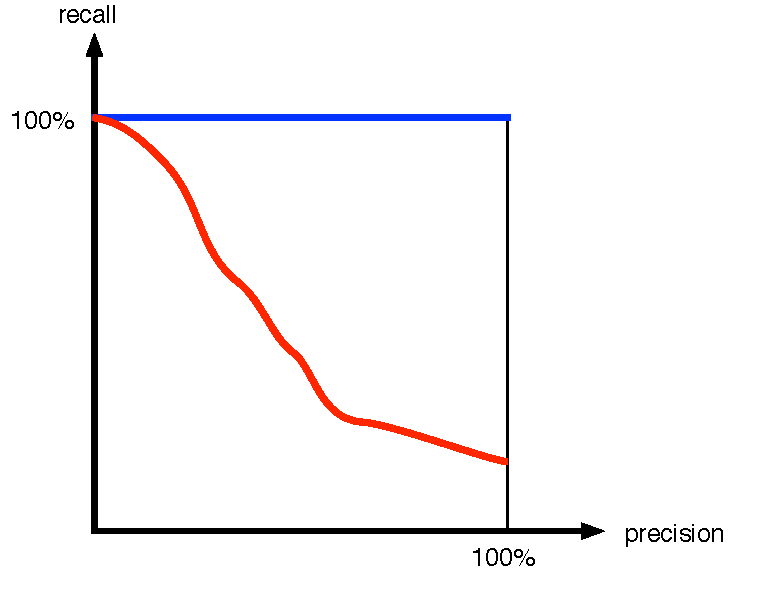
\includegraphics[width=0.6\textwidth]{prc}
\caption{Precision-recall (PR) curves.  In blue is the performance of an ideal classifier and in red is the performance of an imperfect classifier.}
\label{fig:prc}
\end{figure}


We mentioned above about the classifier being conservative or permissive but in fact classifiers lie along a continuous spectrum between these two extremes.
A binary classifier's output is based on the input data and some decision boundary (or discrimination threshold) which might be a simple threshold test or the margin in a support vector machine (SVM).
As we adjust the threshold the precision and recall of the classifier will vary.

A precision-recall (PR) curve is simply a plot of recall against precision for a given experiment as the decision threshold is varied.
An example PR curve is shown in Figure \ref{fig:prc}.
The ideal classifier is shown in blue -- at 100\% precision (perfect classification) it has 100\% recall (every positive is returned).
A more realistic classifier is shown in red.  At 0\% precision it returns 100\% of correct classifications but also a huge number of misclassifications.
At 100\% precision it returns only a small fraction of correct classifications.
In practice the PR curve would be computed for a certain number of threshold values and the results interpolated.

For the aircraft passenger screening example above we can compute precision and recall
\[
P = \frac{0}{0+0} =0, \,\,\, R = \frac{0}{0+19} = 0
\]
which are both zero (technically $P$ is undefined).
%In Information Retrieval tasks with binary classification (relevant or not relevant), precision is the fraction of retrieved instances that are relevant, while recall is the fraction of relevant instances that are retrieved. In the context of Information Retrieval, the precision-recall curve becomes very useful.
%
%
%The precision-recall plot is a model-wide measure for evaluating binary classifiers and closely related to the ROC plot.
%
%
%Important in information retrieval, for instance with respect to recalling relevant webpages, and in robot localization in correctly determining location.
%
%When you perform a search on any search engine, you are looking to find the most relevant material, while minimizing the junk that is retrieved. This is the basic objective of any search engine. Unfortunately getting "everything important" while avoiding "junk" is difficult, if not impossible, to accomplish. 
%
%%This can be illustrated with an example. If I have a database with 100 documents, out of which 60 are relevant to a particular keyword. If my IR system returns a total of 50 documents, out of which 40 are relevant, the precision for this system is [math] \frac{40}{50} = 0.8 [\math] and the recall is [math] \frac{40}{60} = 0.66 [\math]
%%If instead there's another IR system that returns only 10 documents, chances are that atleast  9 of them are relevant. This would increase my precision to 0.9 but decrease it's recall to just 0.15.
%
%to assign each document to one of two categories, "relevant" and "not relevant"
%in navigation the robot is at place X or not
%
%In any binary classification task $C(X, t)$ says whether the item $X$ is in the class or not.
%
% 
%
%
%The performance of a classifier is a 2x2 contingency table � the �confusion matrix� of TP, FP, FN, TN
%� Most classifiers can be varied from �conservative� to �liberal�
%� call a larger number of TPs at the expense of also a larger number of FPs
%� it�s a one-parameter curve 
% 
% If we also know the true classification, the performance of the classifier is a 2x2 contingency table, in this application usually called a confusion matrix.
 
 \subsection{Scalar performance measures}
 We have already discussed how precision and recall alone are insufficient to describe the performance of a classifier.  A useful scalar performance measure
 is the $F_1$ score which is the harmonic mean of precision and recall
 \[
 F_1 = 2\frac{P R}{P+R} = \frac{2\TP}{2\TP+\FP+\FN} 
 \]
 and a high number is best.
 
 For a PR curve a useful scalar measure is  the AUC (area under the precision-recall curve) score.  For an ideal classifer (the blue line in Figure \ref{fig:prc}) this would
 be equal to one, or for a real classifier it would be less than one.

In the deep learning world ``average precision'' scalar measures are used, for example mean average precision or mAP.  There are quite a few variants but they essentially take an average of the precision values for a range of recall values.


\section{Receiver operating characteristic (ROC) }
A closely related concept to the PR curve is the ROC curve which is based on other measures computed from the confusion matrix:
\begin{itemize}
\item Sensitivity or true positive rate
  \[
 \TPR = \frac{\TP}{\TP+\FN}
 \]
  
\item Specificity or true negative rate
 \[
 \SPC = \TNR = \frac{\TN}{\TN+\FP}
 \]
 
 \item Fallout or false positive rate
  \[
 \FPR  = \frac{\FP}{\FP+\TN} = 1 - \SPC
 \]
\end{itemize}
 
\begin{figure}
\centering
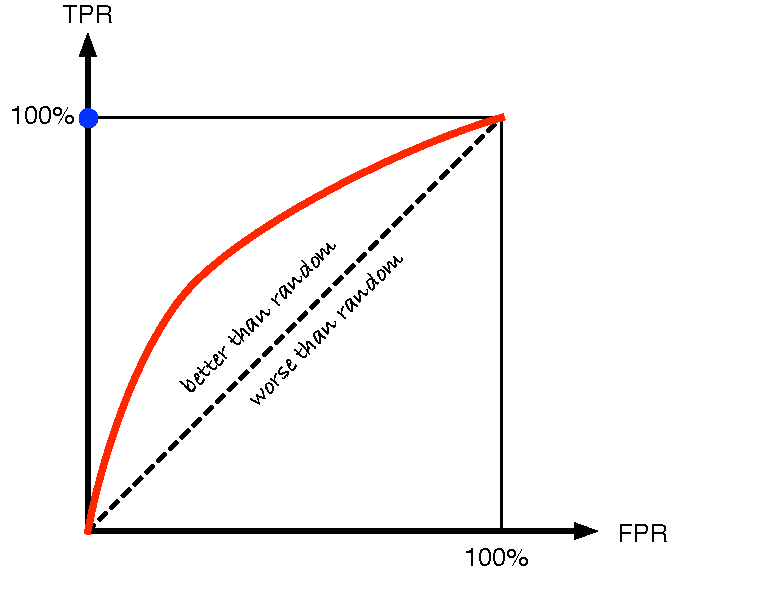
\includegraphics[width=0.6\textwidth]{roc}
\caption{Receiver operating characteristic (ROC) curves.  In blue is the performance of an ideal classifier -- a point.
In red is the performance of an imperfect classifier.  The diagonal line represents the performance of a classifier that makes a random decision, effectively tossing a coin.}
\label{fig:prc}
\end{figure}

The first two, sensitivity and specificity, are commonly used to describe the performance of medical tests.
A plot of $\TPR$ againt $\FPR$ is known as a receiver operating characteristic (ROC) curve\footnote{Developed during WW2 for analysis of radar signals to detect aircraft.}
which is ideally a single point.  The diagonal line is the performance of a random classifier or coin tosser.

There is some argument that PR curves are better for the case where the probability of positives and negatives in the input data, the priors, are important.

% o show this, first let's start with a very nice way to define precision, recall and specificity. Assume you have a "positive" class called 1 and a "negative" class called 0. ? 
%Y
%^
% is your estimate of the true class label Y
%Y
%. Then:
%PrecisionRecall=SensitivitySpecificity=P(Y=1|? =1)=P(? =1|Y=1)=P(? =0|Y=0)
%http://stats.stackexchange.com/questions/7207/roc-vs-precision-and-recall-curves
\bibliographystyle{ieeetr}

\bibliography{mybib}
\end{document}